%%%%%%%%%%%%%%%%%%%%%%%%%%%%%%%%%%%%%%%%
% datoteka diploma-vzorec.tex
%
% vzorčna datoteka za pisanje diplomskega dela v formatu LaTeX
% na UL Fakulteti za računalništvo in informatiko
%
% vkup spravil Gašper Fijavž, december 2010
% 
%
%
% verzija 12. februar 2014 (besedilo teme, seznam kratic, popravki Gašper Fijavž)
% verzija 10. marec 2014 (redakcijski popravki Zoran Bosnić)
% verzija 11. marec 2014 (redakcijski popravki Gašper Fijavž)
% verzija 15. april 2014 (pdf/a 1b compliance, not really - just claiming, Damjan Cvetan, Gašper Fijavž)
% verzija 23. april 2014 (privzeto cc licenca)
% verzija 16. september 2014 (odmiki strain od roba)
% verzija 28. oktober 2014 (odstranil vpisno številko)
% verija 5. februar 2015 (Literatura v kazalu, online literatura)
% verzija 25. september 2015 (angl. naslov v izjavi o avtorstvu)
% verzija 26. februar 2016 (UL izjava o avtorstvu)
% verzija 16. april 2016 (odstranjena izjava o avtorstvu)
% verzija 5. junij 2016 (Franc Solina dodal vrstice, ki jih je označil s svojim imenom)


\documentclass[a4paper, 12pt]{book}

\usepackage[utf8x]{inputenc}   % omogoča uporabo slovenskih črk kodiranih v formatu UTF-8
\usepackage[slovene,english]{babel}    % naloži, med drugim, slovenske delilne vzorce
\usepackage[pdftex]{graphicx}  % omogoča vlaganje slik različnih formatov
\graphicspath{ {images/} }
\usepackage{fancyhdr}          % poskrbi, na primer, za glave strani
\usepackage{amssymb}           % dodatni simboli
\usepackage{amsmath}           % eqref, npr.
%\usepackage{hyperxmp}
\usepackage[hyphens]{url}  % dodal Solina
\usepackage{comment}       % dodal Solina

% Psevdokoda %
\usepackage{amsmath}
\usepackage{algorithm}
\usepackage[noend]{algpseudocode}




\usepackage[pdftex, colorlinks=true,
						citecolor=black, filecolor=black, 
						linkcolor=black, urlcolor=black,
						pagebackref=false, 
						pdfproducer={LaTeX}, pdfcreator={LaTeX}, hidelinks]{hyperref}

\usepackage{color}       % dodal Solina
\usepackage{soul}       % dodal Solina

%%%%%%%%%%%%%%%%%%%%%%%%%%%%%%%%%%%%%%%%
%	DIPLOMA INFO
%%%%%%%%%%%%%%%%%%%%%%%%%%%%%%%%%%%%%%%%
\newcommand{\ttitle}{Simulacija jate ptic}
\newcommand{\ttitleEn}{Flocking simulation}
\newcommand{\tsubject}{\ttitle}
\newcommand{\tsubjectEn}{\ttitleEn}
\newcommand{\tauthor}{Gašper Kolar, Luka Prijatelj}
\newcommand{\tkeywords}{simulacija, jata, ptice, serijski, paralelni, pThreads, OpenMP, OpenCL, MPI}
\newcommand{\tkeywordsEn}{flocking, simulation, serial, parallel, pThreads, OpenMP, OpenCL, MPI}


%%%%%%%%%%%%%%%%%%%%%%%%%%%%%%%%%%%%%%%%
%	HYPERREF SETUP
%%%%%%%%%%%%%%%%%%%%%%%%%%%%%%%%%%%%%%%%
\hypersetup{pdftitle={\ttitle}}
\hypersetup{pdfsubject=\ttitleEn}
\hypersetup{pdfauthor={\tauthor, gk8384@fri.uni-lj.si}}
\hypersetup{pdfkeywords=\tkeywordsEn}


 


%%%%%%%%%%%%%%%%%%%%%%%%%%%%%%%%%%%%%%%%
% postavitev strani
%%%%%%%%%%%%%%%%%%%%%%%%%%%%%%%%%%%%%%%%  

\addtolength{\marginparwidth}{-20pt} % robovi za tisk
\addtolength{\oddsidemargin}{40pt}
\addtolength{\evensidemargin}{-40pt}

\renewcommand{\baselinestretch}{1.3} % ustrezen razmik med vrsticami
\setlength{\headheight}{15pt}        % potreben prostor na vrhu
\renewcommand{\chaptermark}[1]%
{\markboth{\MakeUppercase{\thechapter.\ #1}}{}} \renewcommand{\sectionmark}[1]%
{\markright{\MakeUppercase{\thesection.\ #1}}} \renewcommand{\headrulewidth}{0.5pt} \renewcommand{\footrulewidth}{0pt}
\fancyhf{}
\fancyhead[LE,RO]{\sl \thepage} 
%\fancyhead[LO]{\sl \rightmark} \fancyhead[RE]{\sl \leftmark}
\fancyhead[RE]{\sc \tauthor}              % dodal Solina
\fancyhead[LO]{\sc Diplomska naloga}     % dodal Solina


\newcommand{\BibTeX}{{\sc Bib}\TeX}

%%%%%%%%%%%%%%%%%%%%%%%%%%%%%%%%%%%%%%%%
% naslovi
%%%%%%%%%%%%%%%%%%%%%%%%%%%%%%%%%%%%%%%%  


\newcommand{\autfont}{\Large}
\newcommand{\titfont}{\LARGE\bf}
\newcommand{\clearemptydoublepage}{\newpage{\pagestyle{empty}\cleardoublepage}}
\setcounter{tocdepth}{1}	      % globina kazala

%%%%%%%%%%%%%%%%%%%%%%%%%%%%%%%%%%%%%%%%
% konstrukti
%%%%%%%%%%%%%%%%%%%%%%%%%%%%%%%%%%%%%%%%  
\newtheorem{izrek}{Izrek}[chapter]
\newtheorem{trditev}{Trditev}[izrek]
\newenvironment{dokaz}{\emph{Dokaz.}\ }{\hspace{\fill}{$\Box$}}

%%%%%%%%%%%%%%%%%%%%%%%%%%%%%%%%%%%%%%%%%%%%%%%%%%%%%%%%%%%%%%%%%%%%%%%%%%%%%%%
%% PDF-A
%%%%%%%%%%%%%%%%%%%%%%%%%%%%%%%%%%%%%%%%%%%%%%%%%%%%%%%%%%%%%%%%%%%%%%%%%%%%%%%

%%%%%%%%%%%%%%%%%%%%%%%%%%%%%%%%%%%%%%%% 
% define medatata
%%%%%%%%%%%%%%%%%%%%%%%%%%%%%%%%%%%%%%%% 
\def\Title{\ttitle}
\def\Author{\tauthor, gk8384@fri.uni-lj.si}
\def\Subject{\ttitleEn}
\def\Keywords{\tkeywordsEn}

%%%%%%%%%%%%%%%%%%%%%%%%%%%%%%%%%%%%%%%% 
% \convertDate converts D:20080419103507+02'00' to 2008-04-19T10:35:07+02:00
%%%%%%%%%%%%%%%%%%%%%%%%%%%%%%%%%%%%%%%% 
\def\convertDate{%
    \getYear
}

{\catcode`\D=12
 \gdef\getYear D:#1#2#3#4{\edef\xYear{#1#2#3#4}\getMonth}
}
\def\getMonth#1#2{\edef\xMonth{#1#2}\getDay}
\def\getDay#1#2{\edef\xDay{#1#2}\getHour}
\def\getHour#1#2{\edef\xHour{#1#2}\getMin}
\def\getMin#1#2{\edef\xMin{#1#2}\getSec}
\def\getSec#1#2{\edef\xSec{#1#2}\getTZh}
\def\getTZh +#1#2{\edef\xTZh{#1#2}\getTZm}
\def\getTZm '#1#2'{%
    \edef\xTZm{#1#2}%
    \edef\convDate{\xYear-\xMonth-\xDay T\xHour:\xMin:\xSec+\xTZh:\xTZm}%
}

\expandafter\convertDate\pdfcreationdate 

%%%%%%%%%%%%%%%%%%%%%%%%%%%%%%%%%%%%%%%%
% get pdftex version string
%%%%%%%%%%%%%%%%%%%%%%%%%%%%%%%%%%%%%%%% 
\newcount\countA
\countA=\pdftexversion
\advance \countA by -100
\def\pdftexVersionStr{pdfTeX-1.\the\countA.\pdftexrevision}


%%%%%%%%%%%%%%%%%%%%%%%%%%%%%%%%%%%%%%%%
% XMP data
%%%%%%%%%%%%%%%%%%%%%%%%%%%%%%%%%%%%%%%%  
\usepackage{xmpincl}
\includexmp{pdfa-1b}

%%%%%%%%%%%%%%%%%%%%%%%%%%%%%%%%%%%%%%%%
% pdfInfo
%%%%%%%%%%%%%%%%%%%%%%%%%%%%%%%%%%%%%%%%  
\pdfinfo{%
    /Title    (\ttitle)
    /Author   (\tauthor)
    /Subject  (\ttitleEn)
    /Keywords (\tkeywordsEn)
    /ModDate  (\pdfcreationdate)
    /Trapped  /False
}


%%%%%%%%%%%%%%%%%%%%%%%%%%%%%%%%%%%%%%%%%%%%%%%%%%%%%%%%%%%%%%%%%%%%%%%%%%%%%%%
%%%%%%%%%%%%%%%%%%%%%%%%%%%%%%%%%%%%%%%%%%%%%%%%%%%%%%%%%%%%%%%%%%%%%%%%%%%%%%%

\begin{document}
\selectlanguage{slovene}
\frontmatter
\setcounter{page}{1} %
\renewcommand{\thepage}{}       % preprecimo težave s številkami strani v kazalu
\newcommand{\sn}[1]{"`#1"'}                    % dodal Solina (slovenski narekovaji)

%%%%%%%%%%%%%%%%%%%%%%%%%%%%%%%%%%%%%%%%
%naslovnica
 \thispagestyle{empty}%
   \begin{center}
    {\large\sc Univerza v Ljubljani\\%
      Fakulteta za računalništvo in informatiko}%
    \vskip 10em%
    {\autfont \tauthor\par}%
    {\titfont \ttitle \par}%
    {\vskip 3em \textsc{KONČNO POROČILO\\[5mm]         % dodal Solina za ostale študijske programe
%    VISOKOŠOLSKI STROKOVNI ŠTUDIJSKI PROGRAM\\ PRVE STOPNJE\\ RAČUNALNIŠTVO IN INFORMATIKA}\par}%
    PORAZDELJENI SISTEMI \\ UNIVERZITETNI  ŠTUDIJSKI PROGRAM\\ PRVE STOPNJE\\ RAČUNALNIŠTVO IN INFORMATIKA}\par}%
%    INTERDISCIPLINARNI UNIVERZITETNI\\ ŠTUDIJSKI PROGRAM PRVE STOPNJE\\ RAČUNALNIŠTVO IN MATEMATIKA}\par}%
%    INTERDISCIPLINARNI UNIVERZITETNI\\ ŠTUDIJSKI PROGRAM PRVE STOPNJE\\ UPRAVNA INFORMATIKA}\par}%
%    INTERDISCIPLINARNI UNIVERZITETNI\\ ŠTUDIJSKI PROGRAM PRVE STOPNJE\\ MULTIMEDIJA}\par}%
    \vfill\null%
    %{\large \textsc{Mentor}: doc.\ dr.  Peter Klepec\par}%
   %{\large \textsc{Somentor}:  izr.\ prof.\ dr. Martin Krpan \par}%
    {\vskip 2em \large Ljubljana, 2017 \par}%
\end{center}
% prazna stran
%\clearemptydoublepage      % dodal Solina (izjava o licencah itd. se izpiše na hrbtni strani naslovnice)

% prazna stran
\clearemptydoublepage

%%%%%%%%%%%%%%%%%%%%%%%%%%%%%%%%%%%%%%%%
% kazalo
\pagestyle{empty}
\def\thepage{}% preprecimo tezave s stevilkami strani v kazalu
\tableofcontents{}

% prazna stran
\clearemptydoublepage

%%%%%%%%%%%%%%%%%%%%%%%%%%%%%%%%%%%%%%%%
% povzetek
\addcontentsline{toc}{chapter}{Povzetek}
\chapter*{Povzetek}

\noindent\textbf{Naslov:} \ttitle
\bigskip

\noindent\textbf{Avtor:} \tauthor
\bigskip

%\noindent\textbf{Povzetek:} 
\noindent V vzorcu je predstavljen postopek priprave diplomskega dela z uporabo okolja \LaTeX. Vaš povzetek mora sicer vsebovati približno 100 besed, ta tukaj je odločno prekratek.
\bigskip

\noindent\textbf{Ključne besede:} \tkeywords.
% prazna stran
\clearemptydoublepage


%%%%%%%%%%%%%%%%%%%%%%%%%%%%%%%%%%%%%%%%
\mainmatter
\setcounter{page}{1}
\pagestyle{fancy}

\chapter{Uvod}
Za temo seminarske naloge pri predmetu smo si izbrali simulacijo jate ptic(ang. Flockin simulation).

Vsako iteracijo je potrebno izračunati novo pozicijo za vsako ptico glede na bližnje ptice. Nova pozicija se izračuna glede na 3 preprosta pravila. Ta pravila so ločenost (angl. Separation), usmerjenost (angl. Allignment) in povezanost (angl. Cohesion). Pravilo ločenosti skrbi, da ptice ne letijo pre blizu druga drugi. Pravilo usmerjenosti poskrbi, da ptice v jati letijo v isto smer. Pravilo povezanosti pa poskrbi, da se ptice držijo v jati in ne odletijo vsaka v svojo smer. Stanje vsake ptice je opisano z štirimi komponentami - vektor pozicije (X in Y koordinati) ter vektor smeri oz. hitrosti (X in Y koordinati). 

Iz grobe psevdokode \ref{serial_pseudo_code} algortma je razvidno, da je osnovna serijska implementacija zelo enostavna. Vsako iteracijo se, glede na trenutno stanje, izračuna novo stanje. Novo stanje za vsako ptico se izračuna le glede na lokalne ptice. To so ptice, ki so znotraj določenega radija oddaljenosti od ptice za katero računamo novo stanje. Iskanje lokalnih ptic ima $O(N)$ časovno zahtevnost kjer je $N$ enak številu vseh ptic v jati. Računanje novega stanje za določeno ptico pa ima časovno zahtevnost enako $O(M)$. Tu je $M$ enak številu lokalnih ptic, ki pa ni nikoli večje od $N$ tako, da je časovna zahtevnost računanja novega stanja za določeno ptico prav tako $O(N)$. Novo stanje pa je potrebno izračunati za vse ptice v jati tako, da je časovna zahtevnost celotnega problema enaka $O(N^2)$. 

Iz psevdokode \ref{serial_pseudo_code} se prav tako vidi, da v pomnilniku hranimo le dve tabeli ptic ki jih vsako iteracijo zamenjamo. Prostorska zahtevnost algorima
\begin{algorithm}
\caption{Groba psevdo koda serijskega algoritma}\label{serial_pseudo_code}
\begin{algorithmic}[1]
\State $N \gets \text{Stevilo ptic}$
\State $trenutnoStanje \gets \textit{ptice[N]}$
\State $naslendjeStanje \gets \textit{ptice[N]}$
\Loop
\For{$i \gets 0; i < N; i++$}
\State $lokalnePtice \gets$ poisciLokalnePtice($trenutnoStanje[i], trenutnoStanje);$
\State $naslendjeStanje[i] \gets$ novoStanje($trenutnoStanje[i], lokalnePtice);$
\EndFor
\State izrisiStanje(naslendjeStanje);
\State $trenutnoStanje[i] \gets naslendjeStanje;$
\EndLoop
\end{algorithmic}
\end{algorithm}

\chapter{Serijska implementacija}
\label{ch1}
\section{Osnovna implementacija}
Razvoj osnovne implementacije ni predstavljal večjih izzivov. Za razvoj smo uporabili Microsoftov Visual Studio 2015 integrirano razvojno okolje, ki se je izkazalo za zelo koristno, posebno pri odpravljanju hroščev. Nekoliko težav smo imeli le z grafičnim izrisovanjem jate ptic. Saj smo se avtorji tokrat privič srečali z grafično knjižnico OpenGL. Poleg OpenGL smo uporabili še GLFW knižnjico , ki poskrbi za kreiranje grafičnega okna. Končen rezulatat je prikazan na Sliki~\ref{img:flocking_simulation_demo}. Po približno 10 sekundah leta so se ptice, iz popolnoma naključnih pozicij združile v jate.

Glavna podatkovna struktura programa je $ptica$. $ptica$ zajema vse podatke ki so potrebni za opis ene ptice v prostoru. To sta torej dva dvo-dimenzionalna vektorja $pozicija$ in $smer$. Struktura $jata$ pa združi vse ptice v tabelo $ptic$.

Serijska implementacija potrebuje kot vhodni podatek le število ptic. Glede na število ptic se ustvari ustrezno velika $jata$.

%TODO Dodaj tabelo meritev%
%TODO Dodaj graf meritev%

\begin{figure}[t]
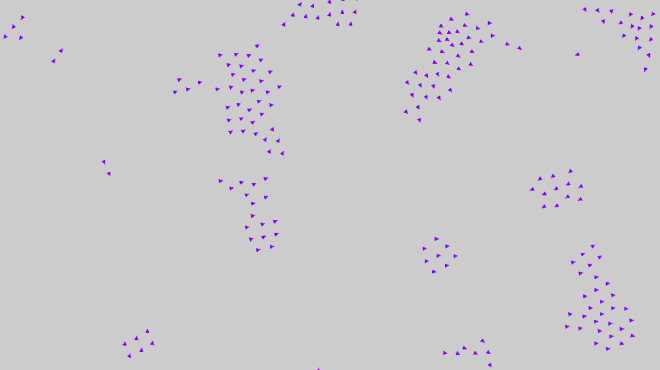
\includegraphics[width=\textwidth]{flocking_simulation_demo}
\caption{Slika je bila zajeta po približno 10 sekundah prostega leta. Ptice so se združile v jate.}
\label{img:flocking_simulation_demo}
\centering
\end{figure}

\section{Implementacija z mrežo}
Zaradi relativno poraznih rezultatov smo se odločili, da serijski algoritem pohitrimo. To smo naredili z implementacijo nove podatkovne strukture mreža (ang. Grid). Iz popravljene psevdokode \ref{serial_grid_pseudo_code} algorirma je razvidno, da se vsako iteracijo ptice najprej razporedi v mrežo na to pa se izračunajo nova stanja ptic. Mreža je ilustrirana na Sliki~\ref{img:flocking_simulation_grid}. Velikost celice je določena z doložino lokalnosti. To je maksimalna razdalja med pticama ki še vedno vplivata druga na drugo. Za računanje novih stanj ptic v neki celici so tako potrebne le ptice v isti in sosednjih celicah. Uporabi se 8-kratna sosednost.

\begin{figure}[t]
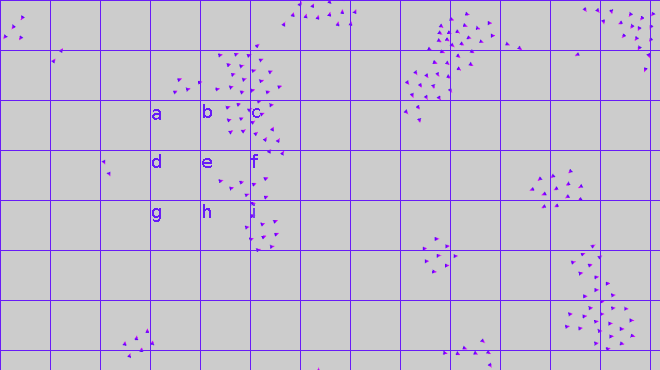
\includegraphics[width=\textwidth]{flocking_simulation_grid}
\caption{Ilustracija mrežne. Za računanje nove pozicije se uporabi 8-kratna sosednjost. To pomeni, da se za izračun novi stanj ptic v celici $e$ upurabijo ptice iz celic $a, b, c, d, e, f, g, h, i$}
\label{img:flocking_simulation_grid}
\centering
\end{figure}

%TODO Vstvi tabelo meritev%
%TODO Vstavi graf meritev%
%TODO Vstavi graf primerjave med navadno in grid%

\begin{algorithm}
\caption{Groba psevdo koda serijskega algoritma z uporabo mreže}\label{serial_grid_pseudo_code}
\begin{algorithmic}[1]
\State $N \gets \text{Stevilo ptic}$
\State $trenutnoStanje \gets \textit{ptice[N]}$
\State $naslendjeStanje \gets \textit{ptice[N]}$
\Loop
\State $mrezaPtic \gets$ razporediPticeVMrezo($trenutnoStanje);$
\For{$i \gets 0; i < N; i++$}
\State $naslendjeStanje[i] \gets$ novoStanje($trenutnoStanje[i], mrezaPtic);$
\EndFor
\State izrisiStanje(naslendjeStanje);
\State $trenutnoStanje[i] \gets naslendjeStanje;$
\EndLoop
\end{algorithmic}
\end{algorithm}

\chapter{Paralelna implementacija z uporabo pThreads}
\label{ch2}
TODO...

\chapter{Paralelna implementacija z uporabo OpenMP}
\label{ch3}
TODO...

\chapter{Paralelna implementacija z uporabo OpenCL}
\label{ch4}
TODO...

\chapter{Paralelna implementacija z uporabo MPI}
\label{ch5}
TODO...


\newpage
\ \\
\clearpage
\addcontentsline{toc}{chapter}{Literatura}
\bibliographystyle{plain}
\bibliography{literatura}


\end{document}

